\clearpage
\section{Telemetry Video}
\label{app:telemetry-video}

The recording command is \texttt{onDesktop/runOperatorVideo}. It starts the same plant run as \texttt{runOperator}, including the initialization datagram of Section~\ref{sec:init-datagram}, and then burns a timing banner into the webcam movie. It uses the clock summary already stored by Appendix~\ref{sec:gpio-clock}. It does not collect a new per-job GPIO or UDP clock map. The September movies in Section~\ref{sec:desktop-clock} used that older map; their one-way split is not what this banner shows.

\subsection{Capture}
Camera name, frame size and timing limits are read from \path{onDesktop/video.json}. The installed file names the camera \texttt{Web Camera}, requests a \(1920\times1080\) frame, and sets
\[
T_{\mathrm{record}}=T_{\mathrm{startup}}+T_{\mathrm{drive}}+T_{\mathrm{tail}}
\]
with \(T_{\mathrm{startup}}=30\)\,s, \(T_{\mathrm{tail}}=2\)\,s and a maximum of 45\,s. The command refuses to start the camera or the controller when \(T_{\mathrm{record}}\) exceeds that maximum. The default drive is 8\,s, so the default recording is 40\,s. A 10\,s drive records 42\,s. \texttt{--duration} sets the drive window, the same window \texttt{runOperator} gives both programs. \texttt{--camera} replaces the camera name for one run. \texttt{--speed} is passed through. The wheels turn unless \texttt{--disable-motors} is present. The robot path remains Wi-Fi \(10.0.0.20\).

The recorder is \path{onDesktop/video/record_timed.swift}. It must print \texttt{RECORDING} before the controller starts. Each saved frame carries the video time and a Desktop \texttt{CLOCK\_MONOTONIC} timestamp. The capture clock is converted through host time onto the same monotonic clock the C++ operator uses, so a banner row can be chosen by comparing that timestamp with the operator event log. The Swift tools are compiled into \path{lineFollowerDistributedBin/} when their sources are newer than the binaries.

After \texttt{runOperator} returns, the script copies the operator record and, from the controller log, the Pi \path{events.csv} and \path{summary.json}. One directory under the repository \path{tmp/video/} holds \path{raw.mp4}, the frame clock, both event logs, \path{overlay.json}, \path{telemetry\_preview.png} and \path{telemetry.mp4}. That directory is the recording. It is not one of the three configuration files kept on the Pi.

\subsection{Banner}
\path{onDesktop/video/prepare_overlay.py} builds one row per recorded frame. \path{overlay_video.swift} draws a 360\,px banner across the bottom of the \(1920\times1080\) frame, with a divider at \(x=920\). The rendered movie begins at the first frame after arming and ends two seconds after the first stop. The longer raw file, including the startup allowance, is left beside it.

The left side follows the latest Desktop decision whose log time is at or before the frame. It shows the local date, the three ADC readings, the signed targets and whether the wheels are enabled, Desktop compute time, transmit latency, the Teensy round trip when a motor acknowledgement exists, and the time since arming. Two lines under that list count commands for the whole job: issued by the Desktop, accepted by the Pi, and confirmed by the Teensy, then how many the Pi replaced before the UART write and how many remain unconfirmed. A missing acknowledgement is not counted as a lost command. Replaced commands are excluded from that remainder.

The right side is fixed for the whole clip. Quartiles use nearest rank: for \(n\) sorted values and fraction \(p\), the reported value is the entry at index \(\lceil np\rceil-1\). Compute time is printed to three decimal places; the other rows use one. Round trip and the sample period are measured without the Desktop clock map, and the renderer draws those two rows in a separate color.

\subsection{Times on the banner}
Desktop compute time is the operator's target time minus the time it received that sample, both on the Desktop monotonic clock.

When \texttt{boot.json} and \texttt{clock\_calib.json} share a hash8, transmit latency is rebuilt for each decision from the same mapping the operator uses. Let \(t_{\mathrm{c}}\) be the Teensy sample-complete time in milliseconds, \(o\) the nominal Pi$-$Teensy offset in milliseconds, \(m\) the median Wi-Fi midpoint in milliseconds, and \(t_{\mathrm{rx}}\) the Desktop receipt time in milliseconds. The mapped completion instant and the transmit latency are
\begin{equation}
t_{\mathrm{D}}=t_{\mathrm{c}}+o+m,
\qquad
\tau=t_{\mathrm{rx}}-t_{\mathrm{D}}.
\label{eq:video-transmit}
\end{equation}
The midpoint \(m\) is a clock origin, as in Section~\ref{sec:init-datagram}. The note under the table is the uncertainty \(u\) of Equation~\eqref{eq:transmit-uncertainty}, and the three columns are the quartiles of \(\tau\).

When the hashes differ, the event log does not keep the per-sample delivery bound. The live transmit number, the first column and the median are then the run median of that bound, and the third column is its 99th percentile. The note says so. Equation~\eqref{eq:video-transmit} is not used for that run.

Round trip uses only the Teensy clock. If \(t_{\mathrm{a}}\) is the ADC start and \(t_{\mathrm{k}}\) is the Teensy time in the motor acknowledgement, both in microseconds,
\begin{equation}
L=(t_{\mathrm{k}}-t_{\mathrm{a}})/1000
\qquad[\mathrm{ms}].
\label{eq:video-round-trip}
\end{equation}
Spare time is the sample period minus \(L\). At the 100\,Hz default the period row is 10.0\,ms in every column. Cycles without a Teensy acknowledgement contribute to the command counts and to compute time, and they leave the round-trip cell blank.

\subsection{Motors-disabled check}
On October 11, 2026, at 13:35 Pacific time, \texttt{runOperatorVideo --duration 8 --disable-motors} recorded the track with the wheels stopped. The drive lasted 7.979\,s after arming. The clock file on the Pi belonged to an earlier boot, so the transmit row is the raw delivery bound: median 5.2\,ms and 99th percentile 6.8\,ms. Desktop compute had quartiles 0.007, 0.009 and 0.011\,ms. Equation~\eqref{eq:video-round-trip} had quartiles 7.1, 7.5 and 8.7\,ms, and the spare quartiles were 1.2, 2.5 and 2.9\,ms. The Desktop issued 777 commands, the Pi accepted 777, the Teensy confirmed 768, the Pi replaced 9 before the UART write, and none remained unconfirmed. Figure~\ref{fig:telemetry-video} is one frame from that movie, two seconds after arming.

\begin{figure}[H]
\centering
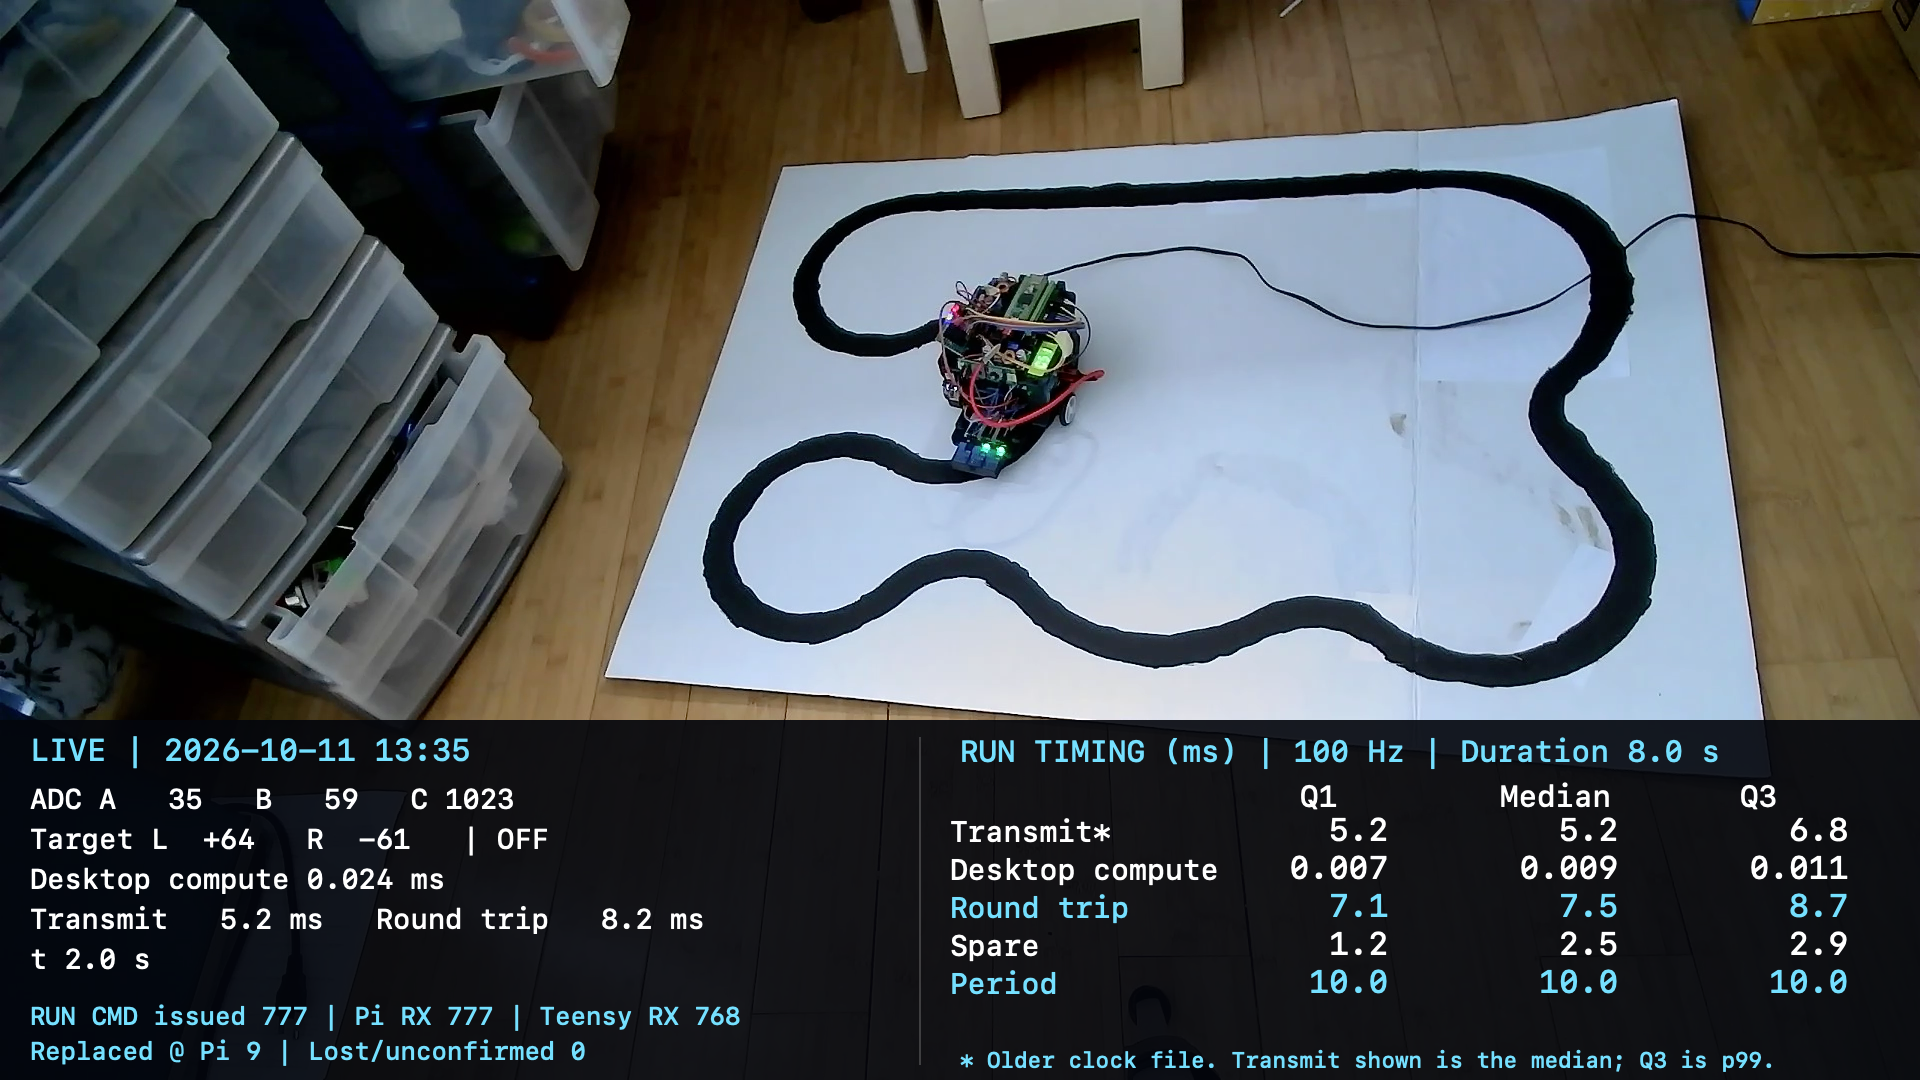
\includegraphics[width=\linewidth]{figures/telemetry_video_preview.png}
\caption{Telemetry frame at \(t=2.0\)\,s from the October 11 motors-disabled recording. The clock hashes did not match, so the transmit row is the raw delivery bound described above. Round trip and spare use the Teensy clock.}
\label{fig:telemetry-video}
\end{figure}
